%%%%%%%%%%%%%%%%%%%%%%%%%%%%%%%%%%%%%%%%%%%%%%%%%%
% MAIN DOCUMENT
%%%%%%%%%%%%%%%%%%%%%%%%%%%%%%%%%%%%%%%%%%%%%%%%%%
\documentclass{thesis}

\title{Thesis Title}
\author{Author Name}
\date{DD Month YYYY}

\begin{document}

%-------------------------------------------------
% FRONT MATTER
%-------------------------------------------------
\pagenumbering{roman}

% TITLE PAGE
%%%%%%%%%%%%%%%%%%%%%%%%%%%%%%%%%%%%%%%%%%%%%%%%%%
% TITLE PAGE
%%%%%%%%%%%%%%%%%%%%%%%%%%%%%%%%%%%%%%%%%%%%%%%%%%
\begin{titlepage}
    \begin{center}
        \large
        \vspace*{.5\baselineskip}
        
            {\Large\scshape University of St. Gallen}
            
            School of Management, Economics, Law, Social Sciences
    
            International Affairs and Computer Science
            
        \vspace{\fill}
            
            Type of Thesis
            
        \vspace{-.5\baselineskip}
            
            \rule{4.25in}{0.5pt}
            
        \vspace{.5\baselineskip}
    
            {\LARGE\scshape\thetitle}
            
            \rule{4.25in}{0.5pt}
    
            \thedate
    
        \vspace{\fill}
            
            \theauthor
            
            Matr.-N\textsuperscript{\underline{\scriptsize o}} 12-345-678
    
            author.email@address.ch
            
            +41 23 456 78 90
    
        \vspace{\fill}
            
            Supervised by
            
            Prof. Dr Supervisor Name
    
        \vspace{\fill}
    \end{center}
\end{titlepage}

% ABSTRACT
\chapter*{Abstract}\label{ch:abstract}
%%%%%%%%%%%%%%%%%%%%%%%%%%%%%%%%%%%%%%%%%%%%%%%%%%
% ABSTRACT
%%%%%%%%%%%%%%%%%%%%%%%%%%%%%%%%%%%%%%%%%%%%%%%%%%

% ACKNOWLEDGEMENTS
\chapter*{Acknowledgements}\label{ch:acknowledgements}
%%%%%%%%%%%%%%%%%%%%%%%%%%%%%%%%%%%%%%%%%%%%%%%%%%
% ACKNOWLEDGEMENTS
%%%%%%%%%%%%%%%%%%%%%%%%%%%%%%%%%%%%%%%%%%%%%%%%%%

% TABLE OF CONTENTS
\tableofcontents

% LIST OF TABLES
\listoftables

% LIST OF FIGURES
\listoffigures

% LIST OF ABBREVIATIONS
\printabbreviations
\setcounter{table}{0} % reset table count since the list of abbreviations is formatted as a longtable
\glsresetall % reset first appearance of abbreviations in case they were used in the abstract

%-------------------------------------------------
% CHATPERS
%-------------------------------------------------
\clearpage
\pagenumbering{arabic}

%%%%%%%%%%%%%%%%%%%%%%%%%%%%%%%%%%%%%%%%%%%%%%%%%%
% CODE SNIPPETS
%%%%%%%%%%%%%%%%%%%%%%%%%%%%%%%%%%%%%%%%%%%%%%%%%%
\newpage

% CROSS-REFERENCES
\section*{Cross-References}
\noindent ref: \ref{ch:introduction} % number

\noindent autoref: \autoref{ch:introduction} % name and number

\noindent pageref: \pageref{ch:introduction} % page number

\noindent autopageref: \autopageref{ch:introduction} % page name and number

% ch:chapter
% sec:section
% subsec:subsection
% fig:figure
% tab:table
% eq:equation
% lst:code-listing
% itm:enumerated-list-item
% alg:algorithm
% app:appendix-subsection

% CITATIONS
\section*{Citations}
\noindent textcite: \textcite[p. 13]{westfahl:space}

\noindent textcites: \textcites[p. 13]{westfahl:space}{angenendt}[p. 13]{baez/article}

\noindent parencite: \parencite[see][p. 13]{westfahl:space}

\noindent parencites: \parencites(see)(and \autoref{ch:introduction})[p. 13]{westfahl:space}{angenendt}[p. 34]{baez/article}

% NOTE: this terminal command checks for uncited references
% checkcites main.aux

% ABBREVIATIONS
\section*{Abbreviations}
\noindent gls: \gls{abbr} % singular

\noindent Gls: \Gls{abbr} % singular capitalised

\noindent glspl: \glspl{abbr} % plural

\noindent Glspl: \Glspl{abbr} % plural capitalised

% FOOTNOTES
\section*{Footnotes}
Lorem ipsum dolor sit amet, consectetur adipiscing elit\footnote{Ut enim ad minim veniam, quis nostrud exercitation ullamco laboris nisi ut aliquip ex ea commodo consequat. Duis aute irure dolor in reprehenderit in voluptate velit esse cillum dolore eu fugiat nulla pariatur.}, sed do eiusmod tempor incididunt ut labore et dolore magna aliqua. Ut enim ad minim veniam, quis nostrud exercitation ullamco laboris nisi ut aliquip ex ea commodo consequat. Duis aute irure dolor in reprehenderit in voluptate velit esse cillum dolore eu fugiat nulla pariatur.\footnote[42]{...is that the answer to everything?}

% ITEMIZE
\section*{Itemize}
\begin{itemize}
    \item Lorem ipsum dolor sit amet, consectetur adipiscing elit, sed do eiusmod tempor incididunt ut labore et dolore magna aliqua.
    \item Ut enim ad minim veniam, quis nostrud exercitation ullamco laboris nisi ut aliquip ex ea commodo consequat.
\end{itemize}

% ENUMERATE
\section*{Enumerate}
\begin{enumerate}
    \item Lorem ipsum dolor sit amet, consectetur adipiscing elit, sed do eiusmod tempor incididunt ut labore et dolore magna aliqua.
    \item Ut enim ad minim veniam, quis nostrud exercitation ullamco laboris nisi ut aliquip ex ea commodo consequat.
\end{enumerate}

% LISTINGS
\section*{Listing}
Lorem ipsum dolor sit amet, \lstinline[style=python]{first_name = "Nora"} consectetur adipiscing elit, sed do eiusmod tempor incididunt ut labore et dolore magna aliqua.

\begin{lstlisting}[style=python]
# This is some sample python code
first_name = "Nora"
favorite_language = "Python"
print(f"Hi, my name is {first_name}. I am learning {favorite_language}.")
\end{lstlisting}

% FIGURE
\section*{Figure}
\begin{figure}[H]
\ffigbox[\textwidth]
    {\caption{Caption}\label{fig:label-1}}
    {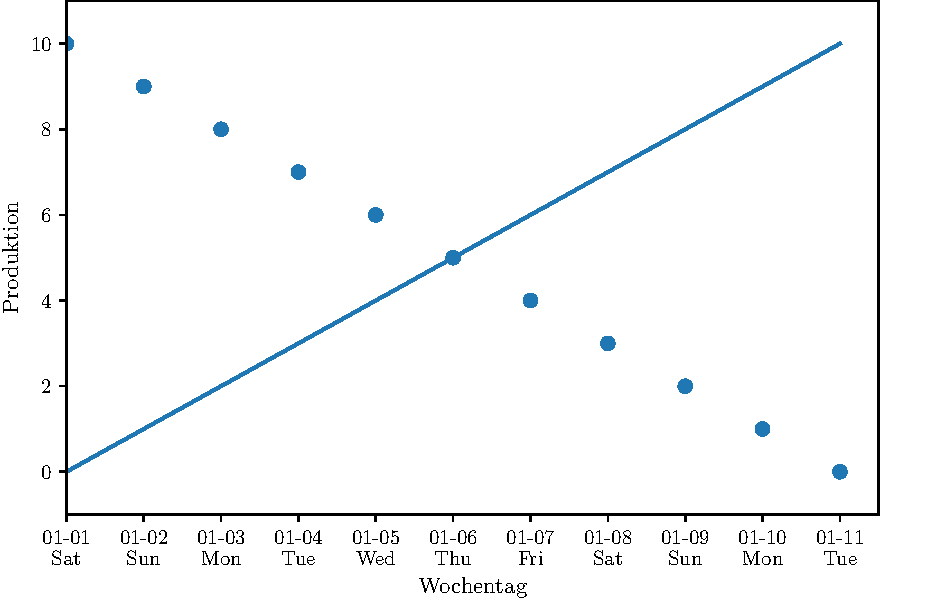
\includegraphics[width=\hsize]{Resources/figure.pdf}
    \floatfoot{Floatfoot.}}
\end{figure}

% TABLE
\section*{Table}
\begin{table}[H]
\ttabbox
    {\caption{Caption}\label{tab:label-1}}
    {\begin{tabular}{@{}cl*{2}{S[table-format=+2.2, round-mode=places, round-precision=2]}l@{}} \toprule
        & & \multicolumn{3}{c}{Measurements} \\ \cmidrule(l){3-5}
        & {Weekday} & {Temperature} & {Percipitation} & {Cloudy} \\ \midrule
        \csvreader[late after line=\\, head to column names, filter={\thecsvinputline<9}]{Resources/data.csv}{}{\thecsvrow & \weekday & \temperature &\percipitation & \cloudy} \midrule
        \csvreader[late after line=\\, head to column names, filter={\thecsvinputline=9}]{Resources/data.csv}{}{& \weekday & \temperature &\percipitation & \cloudy} \bottomrule
    \end{tabular}
    \floatfoot{Floatfoot.}}
\end{table}

% NOTE: \csvautobooktabular{Resources/data.csv} creates automatic table
% NOTE: \thecsvrow returns row number after filter, \thecsvinputline returns row number before filter
% NOTE: \csvcoli is based on roman numerals i.e. it continues at csvrowiv, csvrowv, etc.
% NOTE: if csvsimple cannot find the header of the first column, this is likeley due to LaTeX not ignoring the utf-8 BOM byte order mark U+FEFF: try switching to a different compiler such as XeLaTeX or LuaLaTeX

% FLOATROW
\section*{Floatrow}
\begin{figure}[H]
    \begin{floatrow}
    \ffigbox[\hsize]
        {\caption{Caption}\label{fig:label-2}}
        {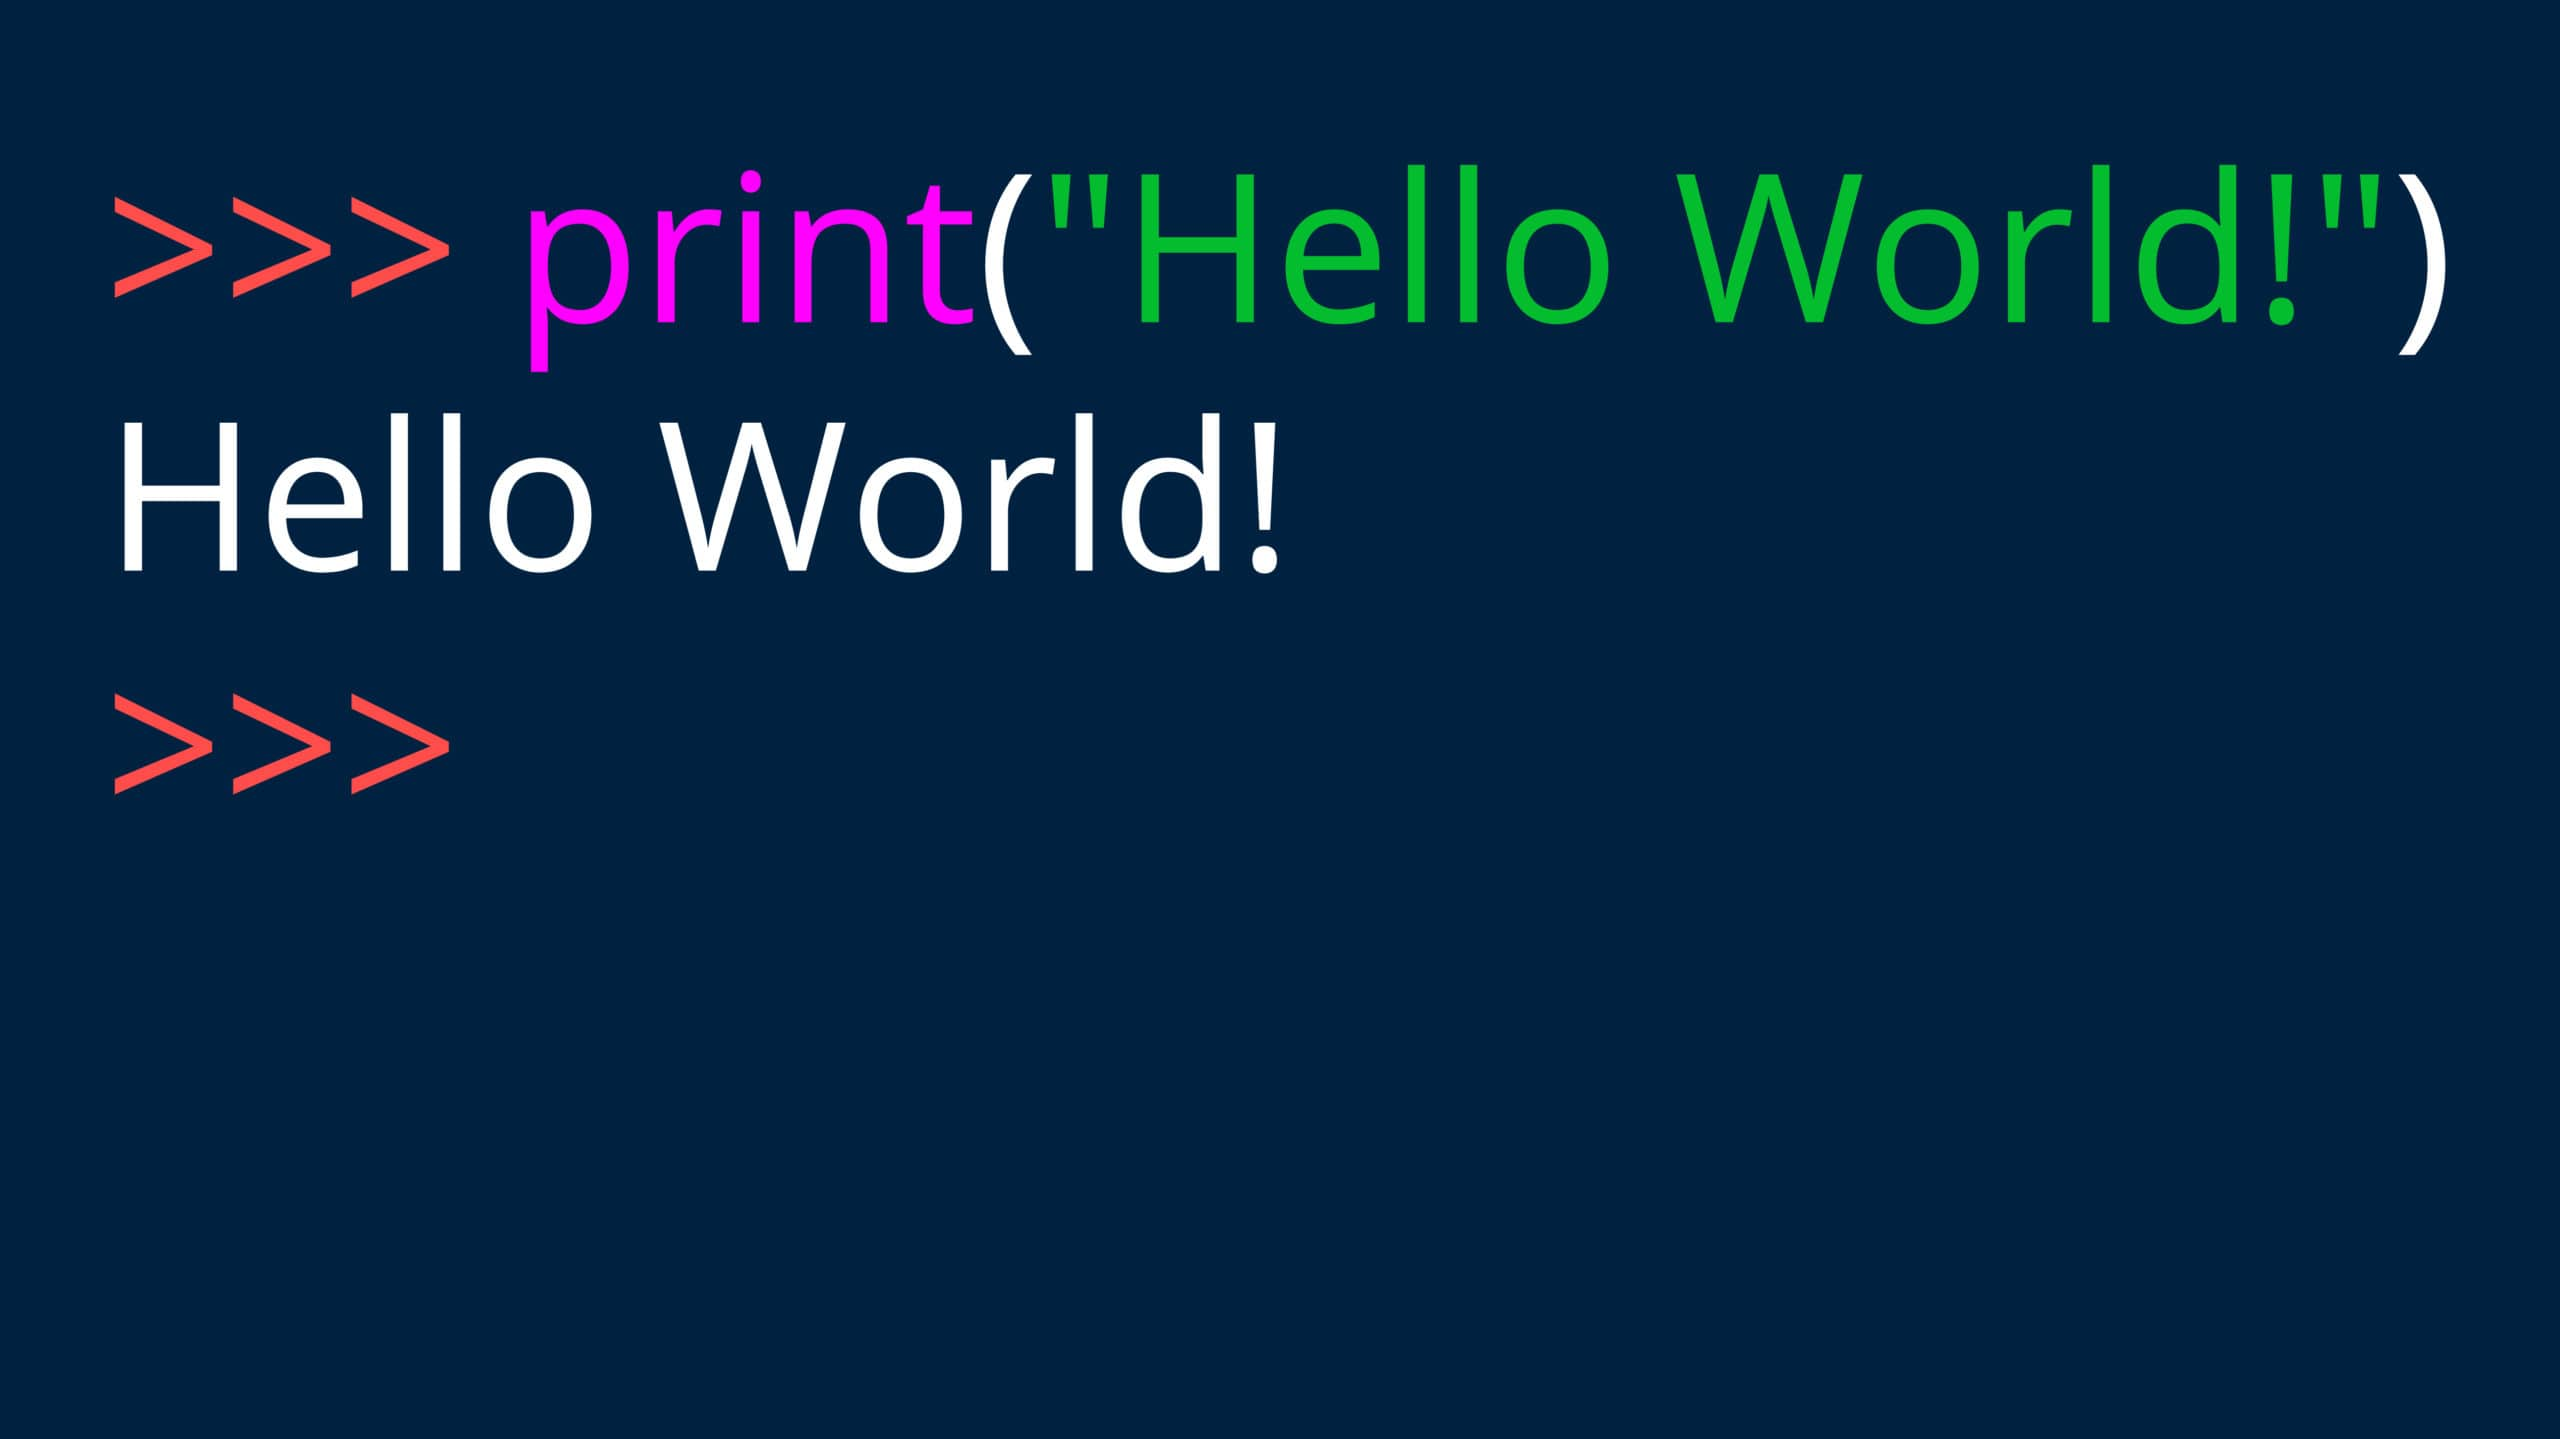
\includegraphics[width=\hsize]{Resources/image.jpeg}
        \floatfoot{Floatfoot.}}
    \ttabbox[\hsize]
        {\caption{Caption}\label{tab:label-2}}
        {\begin{tabular}{@{}lS[table-format=5]S[table-format=3.2]@{}} \toprule
            Datensatz & {Länge (n)} & {Länge (\%)} \\ \midrule % braces escape siunitx formatting
            Training    & 9999  & 99.99 \\
            Validierung & 9999  & 99.99 \\
            Test        & 9999  & 99.99 \\ \midrule
            Total       & 10000 & 100.00 \\ \bottomrule
        \end{tabular}
        \floatfoot{Floatfoot.}}
    \end{floatrow}
\end{figure}

% INTRODUCTION
\chapter{Introduction}\label{ch:introduction}
%%%%%%%%%%%%%%%%%%%%%%%%%%%%%%%%%%%%%%%%%%%%%%%%%%
% CHAPTER 1 - INTRODUCTION
%%%%%%%%%%%%%%%%%%%%%%%%%%%%%%%%%%%%%%%%%%%%%%%%%%
Lorem ipsum dolor sit amet, consectetur adipiscing elit, sed do eiusmod tempor incididunt ut labore et dolore magna aliqua. Ut enim ad minim veniam, quis nostrud exercitation ullamco laboris nisi ut aliquip ex ea commodo consequat. Duis aute irure dolor in reprehenderit in voluptate velit esse cillum dolore eu fugiat nulla pariatur.

\section{Section title}
Lorem ipsum dolor sit amet, consectetur adipiscing elit, sed do eiusmod tempor incididunt ut labore et dolore magna aliqua. Ut enim ad minim veniam, quis nostrud exercitation ullamco laboris nisi ut aliquip ex ea commodo consequat. Duis aute irure dolor in reprehenderit in voluptate velit esse cillum dolore eu fugiat nulla pariatur.

\subsection{Subsection title}
Lorem ipsum dolor sit amet, consectetur adipiscing elit, sed do eiusmod tempor incididunt ut labore et dolore magna aliqua. Ut enim ad minim veniam, quis nostrud exercitation ullamco laboris nisi ut aliquip ex ea commodo consequat. Duis aute irure dolor in reprehenderit in voluptate velit esse cillum dolore eu fugiat nulla pariatur.

\subsubsection{Subsubsection title}
Lorem ipsum dolor sit amet, consectetur adipiscing elit, sed do eiusmod tempor incididunt ut labore et dolore magna aliqua. Ut enim ad minim veniam, quis nostrud exercitation ullamco laboris nisi ut aliquip ex ea commodo consequat. Duis aute irure dolor in reprehenderit in voluptate velit esse cillum dolore eu fugiat nulla pariatur.

\paragraph{Paragraph title}
Lorem ipsum dolor sit amet, consectetur adipiscing elit, sed do eiusmod tempor incididunt ut labore et dolore magna aliqua. Ut enim ad minim veniam, quis nostrud exercitation ullamco laboris nisi ut aliquip ex ea commodo consequat. Duis aute irure dolor in reprehenderit in voluptate velit esse cillum dolore eu fugiat nulla pariatur.

\subparagraph{Subparagraph title}
Lorem ipsum dolor sit amet, consectetur adipiscing elit, sed do eiusmod tempor incididunt ut labore et dolore magna aliqua. Ut enim ad minim veniam, quis nostrud exercitation ullamco laboris nisi ut aliquip ex ea commodo consequat. Duis aute irure dolor in reprehenderit in voluptate velit esse cillum dolore eu fugiat nulla pariatur.

% LITERATURE REVIEW
\chapter{Literature Review}\label{ch:literature-review}
%%%%%%%%%%%%%%%%%%%%%%%%%%%%%%%%%%%%%%%%%%%%%%%%%%
% CHAPTER 2 - LITERATURE REVIEW
%%%%%%%%%%%%%%%%%%%%%%%%%%%%%%%%%%%%%%%%%%%%%%%%%%

% METHODOLOGY
\chapter{Methodology}\label{ch:methodology}
%%%%%%%%%%%%%%%%%%%%%%%%%%%%%%%%%%%%%%%%%%%%%%%%%%
% CHAPTER 3 - METHODOLOGY
%%%%%%%%%%%%%%%%%%%%%%%%%%%%%%%%%%%%%%%%%%%%%%%%%%

% RESULTS
\chapter{Results}\label{ch:results}
%%%%%%%%%%%%%%%%%%%%%%%%%%%%%%%%%%%%%%%%%%%%%%%%%%
% CHAPTER 4 - RESULTS
%%%%%%%%%%%%%%%%%%%%%%%%%%%%%%%%%%%%%%%%%%%%%%%%%%

% DISCUSSION
\chapter{Discussion}\label{ch:discussion}
%%%%%%%%%%%%%%%%%%%%%%%%%%%%%%%%%%%%%%%%%%%%%%%%%%
% CHAPTER 5 - DISCUSSUION
%%%%%%%%%%%%%%%%%%%%%%%%%%%%%%%%%%%%%%%%%%%%%%%%%%

% CONCLUSION
\chapter{Conclusion}\label{ch:conclusion}
%%%%%%%%%%%%%%%%%%%%%%%%%%%%%%%%%%%%%%%%%%%%%%%%%%
% CHAPTER 6 - CONCLUSION
%%%%%%%%%%%%%%%%%%%%%%%%%%%%%%%%%%%%%%%%%%%%%%%%%%

%-------------------------------------------------
% REFERENCES
%-------------------------------------------------
\printbibliography[title=References, heading=bibintoc]

%-------------------------------------------------
% APPENDICES
%-------------------------------------------------
\appendix

% APPENDIX A
\chapter*{Appendix A: Title}\label{ch:appendix-a}
\addcontentsline{toc}{chapter}{Appendix A: Title}
%%%%%%%%%%%%%%%%%%%%%%%%%%%%%%%%%%%%%%%%%%%%%%%%%%
% APPENDIX A - 
%%%%%%%%%%%%%%%%%%%%%%%%%%%%%%%%%%%%%%%%%%%%%%%%%%

% APPENDIX B
\chapter*{Appendix B: Title}\label{ch:appendix-b}
\addcontentsline{toc}{chapter}{Appendix B: Title}
%%%%%%%%%%%%%%%%%%%%%%%%%%%%%%%%%%%%%%%%%%%%%%%%%%
% APPENDIX B - 
%%%%%%%%%%%%%%%%%%%%%%%%%%%%%%%%%%%%%%%%%%%%%%%%%%

% APPENDIX C
\chapter*{Appendix C: Title}\label{ch:appendix-c}
\addcontentsline{toc}{chapter}{Appendix B: Title}
%%%%%%%%%%%%%%%%%%%%%%%%%%%%%%%%%%%%%%%%%%%%%%%%%%
% APPENDIX C - 
%%%%%%%%%%%%%%%%%%%%%%%%%%%%%%%%%%%%%%%%%%%%%%%%%%

% DECLARATION OF AUTHORSHIP
\chapter*{Declaration of Authorship}\label{ch:declaration-of-authorship}
%%%%%%%%%%%%%%%%%%%%%%%%%%%%%%%%%%%%%%%%%%%%%%%%%%
% DECLARATION OF AUTHORSHIP
%%%%%%%%%%%%%%%%%%%%%%%%%%%%%%%%%%%%%%%%%%%%%%%%%%
"I hereby declare,
\begin{itemize}
    \item that I have written this thesis independently;
    \item that I have written the thesis using only the aids specified in the index;
    \item that all parts of the thesis produced with the help of aids have been precisely declared;
    \item that I have mentioned all sources used and cited them correctly according to established academic citation rules;
    \item that I have acquired all immaterial rights to any materials I may have used, such as images or graphics, or that these materials were created by me;
    \item that the topic, the thesis or parts of it have not already been the object of any work or examination of another course, unless this has been expressly agreed with the faculty member in advance and is stated as such in the thesis;
    \item that I am aware of the legal provisions regarding the publication and dissemination of parts or the entire thesis and that I comply with them accordingly;
    \item that I am aware that my thesis can be electronically checked for plagiarism and for third-party authorship of human or technical origin and that I hereby grant the University of St.Gallen the copyright according to the Examination Regulations as far as it is necessary for the administrative actions;
    \item that I am aware that the University will prosecute a violation of this Declaration of Authorship and that disciplinary as well as criminal consequences may result, which may lead to expulsion from the University or to the withdrawal of my title."
\end{itemize}

\noindent By submitting this thesis, I confirm through my conclusive action that I am submitting the Declaration of Authorship, that I have read and understood it, and that it is true.

\vspace{\baselineskip}
\centering
\begin{tabular}{ccc}
    & & 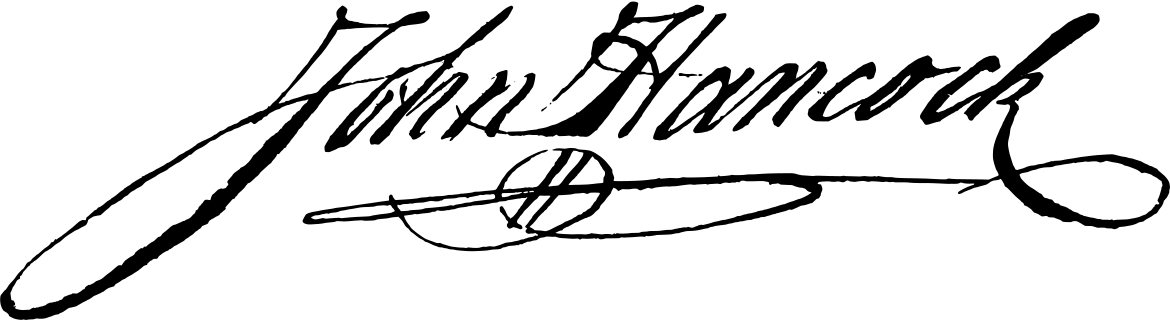
\includegraphics[width=1.75in]{Resources/signature.png} \\ [-.6in]
    \large DD.MM.YYYY & & \\ [-2.5ex]
    \makebox[1.25in]{\hrulefill} & \makebox[1.25in]{} & \makebox[1.25in]{\hrulefill} \\ [-1ex]
    Date & & Signature
\end{tabular}

\end{document}